\documentclass[a4paper,twoside,12pt]{report}
% Richard Klein (2020,2021)

% Include Packages
%\usepackage[a4paper,inner=3.5cm,outer=2.5cm,top=2.5cm,bottom=2.5cm]{geometry}  % Set page margins
\usepackage{fullpage}
\usepackage{float}                  % Allows 'Here and Only Here' [H] for Floats
\usepackage{url}                    % \url{} command
\usepackage{charter}                  % Set font to Times
\usepackage{graphicx}               % \includegraphics
\usepackage{subfigure}              % Allow subfigures
\usepackage{amsmath}
\usepackage{amssymb}
\usepackage{amsthm}
\usepackage{booktabs}
\usepackage{parskip}
\usepackage[all]{nowidow}
\setnoclub[2]
\setnowidow[2]

% Referencing
% Provides \Vref and \vref to indicate where a reference is.
\usepackage{varioref} 
% Hyperlinks references
\usepackage[bookmarks=true,bookmarksopen=true]{hyperref} 
% Provides \Cref, \cref, \Vref, \vref to include the type of reference: fig/eqn/tbl
\usepackage{cleveref} 
% Setup Hyperref
\hypersetup{
  colorlinks   = true,              %Colours links instead of ugly boxes
  urlcolor     = blue,              %Colour for external hyperlinks
  linkcolor    = blue,              %Colour of internal links
  citecolor    = blue                %Colour of citations
}
% Names for Clever Ref
\crefname{table}{table}{tables}
\Crefname{table}{Table}{Tables}
\crefname{figure}{figure}{figures}
\Crefname{figure}{Figure}{Figures}
\crefname{equation}{equation}{equations}
\Crefname{equation}{Equation}{Equations}

% Wits Citation Style
\usepackage{natbib} \input{natbib-add}
\bibliographystyle{named-wits}
\bibpunct{[}{]}{;}{a}{}{}  % to get correct punctuation for bibliography
\setlength{\skip\footins}{1.5cm}
\newcommand{\citets}[1]{\citeauthor{#1}'s \citeyearpar{#1}}
\renewcommand\bibname{References}  

\pagestyle{headings}

\pagestyle{plain}
\pagenumbering{roman}

\renewenvironment{abstract}{\ \vfill\begin{center}\textbf{Abstract}\end{center}\addcontentsline{toc}{section}{Abstract}}{\vfill\vfill\newpage}
\newenvironment{declaration}{\ \vfill\begin{center}\textbf{Declaration}\end{center}\addcontentsline{toc}{section}{Declaration}}{\vfill\vfill\newpage}
\newenvironment{acknowledgements}{\ \vfill\begin{center}\textbf{Acknowledgements}\end{center}\addcontentsline{toc}{section}{Acknowledgements}}{\vfill\vfill\newpage}

\begin{document}
\onecolumn
\thispagestyle{empty}

\setcounter{page}{0}
\addcontentsline{toc}{chapter}{Preface}
\ 
\begin{center}
  \vfill
  {
  \huge \bf \textsc{The Development of Cyber Threat Intelligence System Framework for the Mining Industry}\\
  \rule{\linewidth}{0.5pt}

%   \large Subtitle\\[20pt]


  \normalsize
  Proposed by:\\
  MUHAMMAD UMER FAROOQ\\
  2925331\\[20pt]
  Supervisors:\\[10pt]
  Dr. Helen Robertson\\[10pt]
  Dr. Ahsan Mahboob\\[10pt]
  \today
  }
  \vfill

  \vfill
  
\includegraphics[width=2.5cm]{images/wits.png}
  \vfill
  \vfill

%   \vspace{10pt}\\
  % \small{Ethics Clearance Number: XX/XX/XX}\\[10pt]
  \small{A proposal submitted to the Faculty of Science, University of the Witwatersrand, Johannesburg,
in partial fulfilment of the requirements for the degree of Master of Science (Dissertation) in Computer Science}\\
\rule{\linewidth}{0.5pt}
\large School of Computer Science \& Applied Mathematics\\
\large University of the Witwatersrand\\[20pt]

\end{center}
\vfill
\newpage

\pagestyle{plain}
\setcounter{page}{1}

\phantomsection
\begin{abstract}
The mining industry's growing reliance on digital technologies has significantly increased its vulnerability to cyber threats, which can lead to severe operational, financial, and environmental consequences. This research aims to develop a comprehensive Cyber Threat Intelligence (CTI) system tailored specifically for the mining sector, utilizing advanced data analytics and machine learning to enhance cyber threat detection and mitigation capabilities. A mixed-methods approach combining systematic literature reviews, empirical testing, and qualitative analyses ensures a robust framework that addresses both technical and ethical considerations. The proposed CTI system will gather, aggregate, and analyze data from diverse sources, such as network logs and open-source intelligence feeds, employing machine learning techniques to identify patterns and anomalies indicative of cyber threats. This research also critically examines the ethical implications of deploying such systems, ensuring compliance with industry standards and regulations. By integrating stakeholder feedback throughout the development and implementation phases, the study ensures that the CTI system is practical, effective, and aligned with the mining industry’s specific needs. The anticipated outcomes include improved resilience against cyber threats, minimized risk of operational disruptions, and enhanced protection of sensitive data and infrastructure. This research contributes to the broader field of cybersecurity in critical infrastructure, providing valuable insights into the application of CTI systems within industry-specific contexts.
\end{abstract}

\phantomsection
\begin{declaration}
I, Muhammad Umer Farooq, hereby declare the contents of this research proposal to be my own work.
This proposal is submitted for the Master of Science by Dissertation in Computer Science at the University of the Witwatersrand.
This work has not been submitted to any other university, or for any other degree.
\end{declaration}

\phantomsection
\begin{acknowledgements}
I would like to express my deepest gratitude to my supervisors, Dr. Helen Robertson from the School of Computer Science and Mathematics, and Dr. M. Ahsan Mahboob, the Head of Sibanye Stillwater Digital Mining Laboratory (DigiMine), for their invaluable guidance and support throughout my research journey. I would like to thatnk and acknowledge the financial support provided by the Sibanye-Stillwater Digital Mining Laboratory (DigiMine), Wits Mining Institute (WMI).

Dr. Robertson’s expertise and insightful feedback were instrumental in refining my work, and her encouragement was a constant source of motivation. I am equally grateful to Dr. Mahboob for his mentorship and for providing me with the opportunity to collaborate within the DigiMine lab, where his leadership and profound knowledge in the field greatly enhanced my research experience.

Their unwavering support, constructive feedback, and encouragement have been crucial to the successful completion of this proposal. I am deeply appreciative of their time and efforts, and I feel privileged to have worked under their guidance.
\end{acknowledgements}


\phantomsection
\addcontentsline{toc}{section}{Table of Contents}
\tableofcontents
\newpage
\phantomsection
\addcontentsline{toc}{section}{List of Figures}
\listoffigures
\newpage
\phantomsection
\addcontentsline{toc}{section}{List of Tables}
\listoftables
\newpage
\pagenumbering{arabic}
% Chapter 1
\chapter{Introduction}
The Mining Industry is as important part of the global economy. It depends on digital technologies to improve operations, safety, and sustainability. However, this reliance on technology exposes the industry to significant cyber threats that can disrupt operations, compromise safety, and cause financial loss and environmental harm. Given these risks, the need for effective cyber threat detection in mining is more urgent than ever. Traditional and reactive cybersecurity measures often fail to address the complex and evolving threats specific to the mining sector. This has led to the growing importance of Cyber Threat Intelligence (CTI) System for the mining sector, which proactively detect, analyze, and respond to potential threats using intelligence feeds. These systems collect and analyze data from multiple sources, helping organizations identify and mitigate risks before they cause damage. Despite potential threats, the urgency for effective cyber threat detection in mining has never been greater. Traditional reactive cybersecurity measures used in the sector often fall short of addressing the sophisticated and evolving threats unique to the mining sector. This research aims to fill these gaps by developping tailored Cyber Threat Intelligence System Framework specifically for the mining industry. The CTI Framework will use advanced data analytics and machine learning algorithms to detect patterns and anomalies in threats datam and it will improve the industry’s ability to defend against cyber-attacks. Additionally, this study will examine the ethical implications of implementing such a system, ensuring it meets both technical and ethical standards. By designing a CTI system tailored to the mining sector, this research will address a critical need and contribute to the broader field of cybersecurity. In Figure: \ref{fig:thing1}, World Economic Forum Global Risks Perception Survey 2023-2024 indicating a wide subset of the global population to potential digital and physical exploitation.

\begin{figure}[ht]
    \centering
    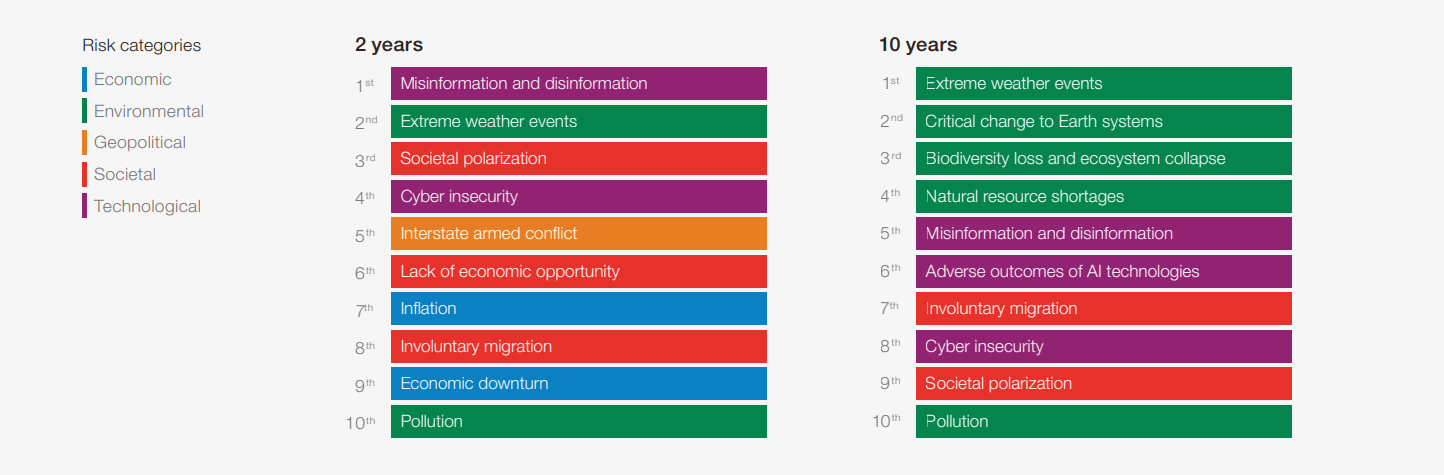
\includegraphics[width=1.0\linewidth]{images/world-economic-forum-global-risks.png}  % If located in the "images" folder
    \caption{World Economic Forum Global Risks Analysis Survey 2023-2024}
    \label{fig:thing1}
\end{figure}

\section{Problem Statement}
Mining Industry plays a crucial role in global economic development. Mining operations are adopting digital technologies rapidly to enhance productivity, safety, and efficiency. These are becoming more vulnerable to cyber threats. These threats can disrupt operations, can compromise sensitive data, can cause financial loss, and even it can endanger lives and the environment. Evolution Mining is an Australian gold mining company. It suffered a ransomware attack in August 2024 on its IT systems, which, though swiftly contained, underscored the industry's susceptibility to cyber threats. A month earlier, in July 2024, Sibanye-Stillwater also faced a cyberattack, leading to temporary IT system outages and manual processing in some of its operations. Norsk Hydro is a major metals and mining company. It experienced a ransomware attack in 2020 that caused significant operational shutdowns and millions in losses.
An attack on a South American in 2017 on a mining firm compromised sensitive geological data. An Australian mining company suffered unauthorized access in 2019 which disrupted automated processes and risked worker safety.
These incidents highlight the urgent necessity for robust, proactive cybersecurity measures to protect the industry from evolving threats.


% 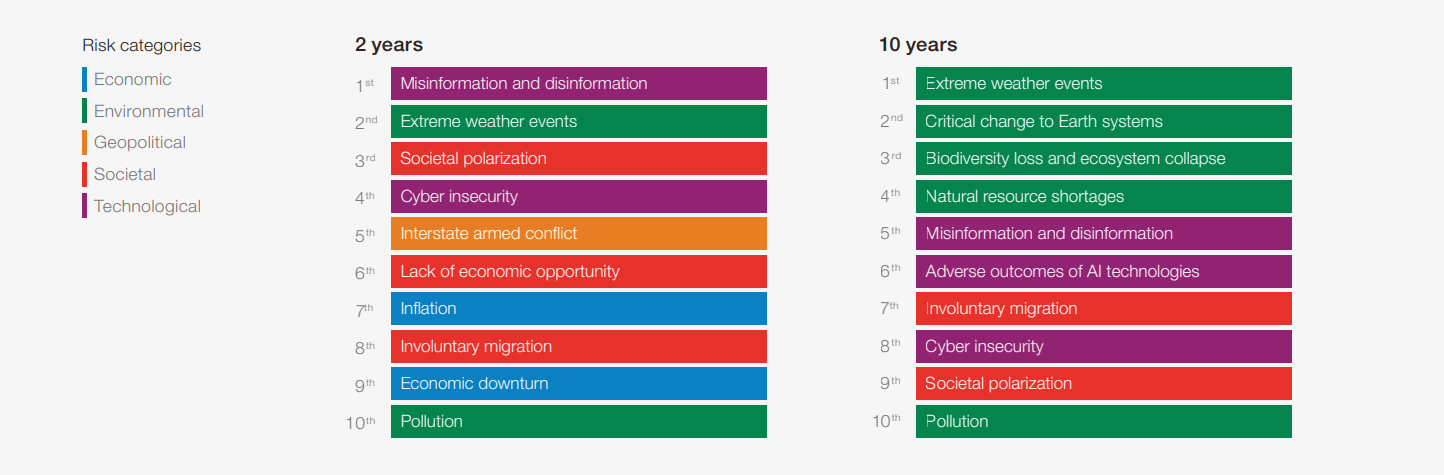
\includegraphics[width=1.0\linewidth]{images/world-economic-forum-global-risks.png}  % If located in the "images" folder
% \caption{World Economic Forum Global Risks Perception Survey 2023-2024}



\section{Research Questions}
% \section{Research Questions}

The following questions are formulated to guide the research for development of a Cyber Threat Intelligence (CTI) system tailored for the mining industry:

\begin{enumerate}
    \item {How can a framework for a Cyber Threat Intelligence (CTI) system be developed specifically for the mining industry?}
 \item {What strategies and technologies can be utilized to efficiently collect, aggregate, and analyze cyber threat data from sources like network logs and open-source intelligence feeds for the mining industry?}

    \item {How can advanced data analysis and machine learning techniques be applied to detect and analyze patterns and anomalies in cyber threat data specific to the mining sector?}

    \item {What are the ethical challenges associated with implementing a CTI system in the mining industry, and how can these be effectively addressed to align with ethical standards and regulations?}
\end{enumerate}
\section{Research Aims and Objectives}
The adoption of digital technologies in the mining industry is essential for advancing productivity and safety. But it has also led it to significant cyber vulnerabilities. Cyber threats continuing to evolve. So, the need for a proactive approach to identify, analyze, and mitigate risks has become essential. The research aims and objectives focus on developing a robust CTI system Framework.\\
\subsection{Research Aims}
The primary aim of this research is to develop an effective Cyber Threat Intelligence (CTI) framework for the mining industry, designed to enhance cybersecurity resilience. This research aims to mitigate the increasing cyber threat risks within the mining industry, which has seen a sharp rise in digital vulnerabilities as it adopts more advanced technologies by developing a CTI Framework tailored to mining industry. This aim involves creating a specialized CTI system that can detect and respond to cyber threats, ensuring the safety, security, and continuity of mining operations in an increasingly digitalized environment.
\subsection{Research Objectives}

The objectives of this research are as follows:

\begin{itemize}
    \item Develop a framework for a Cyber Threat Intelligence (CTI) System tailored specifically to the mining industry.
    \item To collect, aggregate, and analyze threat data from various sources, including network logs and open-source intelligence feeds.
    \item To apply advanced data analysis and machine learning techniques to identify patterns and anomalies within the collected threat data.
    \item To examine and address the ethical considerations and implications of implementing a CTI framework within the mining industry.
\end{itemize}
\section{Limitations}
The basic limitation of this research is the generalizability of its findings across the diverse operational environments within the mining industry. While the study aims to develop a robust Cyber Threat Intelligence (CTI) Framework tailored to mining, it relies on specific datasets and threat scenarios that may not comprehensively reflect all real-world contexts. Differences in mining operations, network architectures, and data characteristics across various geographical and organizational settings could impact the performance and applicability of the CTI framework. Additionally, the effectiveness of the proposed data analysis and machine learning techniques in detecting threats and enhancing model interpretability may vary depending on the complexity and heterogeneity of cyber threat data across mining entities. Consequently, while the research aspires to make valuable contributions to the mining sector's cybersecurity capabilities, its application to the broader landscape of mining operations may be constrained.\\
\section{Overview}


% \subsubsection{This is a subsubsection}
% This is just a paragraph
% \subsection{A Subsection about Citation Style}
% Citations are important. Citation style for Computer Science is:
% \begin{itemize}
% \item When used in the text, use the authors with the date in brackets:\\ \citet{klein17} say very important things.
% \item When used as a reference after a face, put everything in brackets:\\ Import things are true \citep{klein17}.
% \end{itemize}

% \subsection{Compiling}
% Remember to compile multiple times to resolve references. Usually:
% \begin{verbatim}
% pdflatex file.tex
% bibtex file
% pdflatex file.tex
% pdflatex file.tex
% \end{verbatim}

% Chapter 2
\chapter{Background and Literature Review}
\section{Introduction}
This chapter presents the background and literature review essential for developing a Cyber Threat Intelligence (CTI) framework tailored specifically for the mining industry. As industries become increasingly digitalized, the mining sector has not remained isolated from growing cybersecurity risks. This chapter begins by exploring the fundamental concepts of CTI systems and examines current approaches to cybersecurity in industrial sectors with a focus on mining. It discusses methods for collecting and analyzing cyber threat data, such as network logs and open-source intelligence, which are crucial for understanding the threat landscape specific to mining operations.

A key objective of this research is to investigate advanced data analysis and machine learning techniques that can improve the detection of patterns and anomalies in cyber threats. The literature review assesses relevant studies that address these techniques within industrial contexts, including those applicable to mining. Finally, this chapter also critically examines ethical considerations in implementing a CTI framework, acknowledging the importance of aligning with ethical standards and regulations to ensure both data security and industry compliance. These topics collectively provide the foundation for addressing the research questions and objectives, setting the stage for a comprehensive, ethically-sound CTI system for the mining industry.
\subsection{Background}
Cybersecurity initiatives play a crucial role in strategic decision-making within Industry 4.0, aligning digital operations with sustainable solutions \citet{medoh2022future}. The integration of advanced computing, communication technologies, and IoT-cloud infrastructure into critical systems like the Smart Grid and industrial cyber-physical systems (CPS) has introduced significant cybersecurity challenges. The Smart Grid, designed to enhance power system efficiency and reliability, now faces vulnerabilities due to the extensive interconnection of electronic devices, which impacts infrastructure stability and security. Similarly, industrial CPSs—including systems for the mining industries—rely on SCADA for infrastructure monitoring and control, yet traditional SCADA lacks adequate security measures for the complexities of IoT-cloud integration. This transformation exposes critical infrastructures to cyber threats, demanding updated countermeasures, secure protocols, and extensive research to address evolving vulnerabilities in these next-generation systems \citet{wang2013cyber} and \citet{sajid2016cloud}.

\subsection{Related Work}
% Chapter 3
\chapter{Research Methodology}
\section{Research design}
\section{Methods}The research will follow a comprehensive, multi-phase approach tailored to address the
unique cybersecurity challenges encountered by the mining industry. The process will begin
with a requirements analysis, which will involve collecting stakeholder opinions and reviewing
relevant literature to identify specific needs and gaps in current cybersecurity frameworks.
Then, during the framework development phase, a customized architecture will be developed,
integrating data from various sources, such as network logs and open-source intelligence
feeds. Following this, real-time threat data will be collected and aggregated, which will then
be analyzed using advanced machine learning techniques like to detect patterns, classifying
and clustering the logs and anomalies. Ethical considerations will be carefully examined to
ensure compliance with industry regulations and data privacy standards. A prototype of the
CTI System will be developed and tested in a controlled environment to evaluate its
effectiveness. Then, the system’s performance will be assessed, and detailed documentation
will be prepared, offering insights and recommendations for practical implementation within
the mining industry.

\subsection{Pre-Modelling Phase}
The pre-modelling phase focuses on the initial setup and preparation needed to build an effective Cyber Threat Intelligence (CTI) system. It includes data collection, data preprocessing, and defining the threat intelligence goals specific to the mining industry.

\begin{itemize}
    \item \textbf{Data Collection}: Raw data is collected from various sources such as network logs, open-source intelligence (OSINT) feeds, and vendor-specific threat intelligence reports. In mining operations, sensor and operational data can also be leveraged to detect abnormal patterns in the network.
    \item \textbf{Data Preprocessing}: The collected data is cleaned and transformed into a usable format. This involves handling missing data, removing duplicates, and normalizing data formats. Feature extraction techniques such as Principal Component Analysis (PCA) can be applied to reduce noise.
    \item \textbf{Data Labeling}: For supervised learning, historical data is labeled by domain experts as normal or malicious based on past incidents.
    \item \textbf{Goal Definition}: Specific objectives are defined, such as detecting ransomware, Advanced Persistent Threats (APTs), or insider threats, which will influence the models and algorithms chosen in the next phase.
\end{itemize}

\subsection{Modelling Phase}
The modelling phase involves building machine learning models that predict and detect cyber threats based on the pre-processed data.

\begin{itemize}
    \item \textbf{Model Selection}: Machine learning models such as decision trees, random forests, support vector machines (SVMs), or neural networks are selected based on the data type and threat scenarios.
    \item \textbf{Feature Engineering}: Relevant features are engineered to improve the model’s ability to detect cyber threats. Time-series analysis may be used for real-time threat detection in operational environments.
    \item \textbf{Model Training}: Models are trained using supervised learning on labeled data or unsupervised learning on unlabelled data to detect anomalies. Cross-validation techniques are used to avoid overfitting.
    \item \textbf{Threat Classification}: The trained model is used to classify network activity or system behavior into predefined threat categories (e.g., malware, phishing, Denial of Service attacks).
\end{itemize}

\subsection{Post-Modelling Phase}
After building the models, the post-modelling phase focuses on evaluation, validation, and deployment.

\begin{itemize}
    \item \textbf{Model Validation}: Models are validated using test datasets. Key performance metrics such as accuracy, precision, recall, and F1 score are used to measure the model’s effectiveness.
    \item \textbf{Model Tuning}: Hyperparameter tuning (e.g., grid search or random search) is used to optimize the model. This process involves adjusting key parameters to improve performance.
    \item \textbf{Deployment Readiness}: Once validated, the model is integrated into existing systems (e.g., Security Information and Event Management systems) for real-time threat detection. The model undergoes stress testing to ensure it can handle real-time data streams.
\end{itemize}

\subsection{Experimental Setup}
The experimental setup defines how the CTI models are tested in a controlled environment before full deployment.

\begin{itemize}
    \item \textbf{Test Environment Setup}: A simulated or controlled mining network is created, including virtual machines, network traffic simulators, and log generators to mimic realistic scenarios.
    \item \textbf{Data Injection}: Historical data and simulated attack data are injected into the system to evaluate its ability to detect and respond to various threats.
    \item \textbf{Performance Measurement}: The system’s performance is measured using metrics such as detection rate, false alarm rate, and response time. Resource usage (CPU, memory) is also monitored to ensure scalability.
    \item \textbf{Comparison with Existing Systems}: The CTI framework’s performance is compared to existing cybersecurity systems in the mining industry to assess improvements.
\end{itemize}

\subsection{Optimization and Training Models}
The optimization and training phase focuses on refining the models to maximize their performance and efficiency.

\begin{itemize}
    \item \textbf{Hyperparameter Optimization}: Techniques such as grid search or Bayesian optimization are used to identify the best hyperparameters (e.g., learning rates, kernel functions) to improve detection accuracy.
    \item \textbf{Continuous Learning}: As new threats emerge, the model is retrained with updated data. Incremental learning or transfer learning methods may be used to update the model without complete retraining.
    \item \textbf{Efficiency Optimization}: The model is optimized for real-time performance through techniques such as model pruning, quantization, or the use of lightweight architectures.
    \item \textbf{Final Model Training}: The final optimized model is trained on the entire dataset to ensure robustness and accuracy. It is then ready for deployment into the CTI system.
\end{itemize}

\section{Limitations}
\section{Ethical Considerations}


% Chapter 4
\chapter{Schedule of Work}
% Chapter 5
\chapter{Conclusion}
The CTI System for the Mining Industry aims to bridge the gap between the mining industry's unique operational demands and the growing need for robust cybersecurity measures. By developing a tailored CTI System, the study seeks to provide an architecture design of a CTI System. The development of the CTI System will enhance the ability to detect and respond to cyber threats proactively in the mining industry. The CTI System's integration of advanced data analytics and machine learning will offer more precise and real-time action against evolving threats. Additionally, this research will address ethical and regulatory concerns and ensure the proposed solution is effective and compliant with mining industry standards.
The findings from this research will contribute significantly to both the mining industry and the broader field of cybersecurity. By providing a specialized system for cyber threat intelligence, this study will help safeguard critical mining operations, protecting both assets and the environment. The lessons learned and the methodologies developed can serve as a model for other industries facing similar cybersecurity challenges, marking a step forward in the ongoing effort to secure vital industrial infrastructure.



% \LaTeX\ decides how to place images. It also does the referencing for you as seen in \Cref{fig:thing1}. If you have subimages, they should have their own captions and labels -- look into the subfig or subfigure packages.

% Including the image with correct file extension


% Figure captions are at the bottom. Table titles are at the top of the table as seen in \Vref{tab:tab1}. 

% \begin{table}[p]
%   \centering
%   \caption{Table Name}
%   \label{tab:tab1}
%   \begin{tabular}{cc}
%       \hline
%       Col1 & Col2\\
%       \hline\hline 
%       R0,C0 & R0,C1 \\ 
%       R1,C0 & R1,C1 \\ 
%       \hline
%   \end{tabular} 
% \end{table}

% \chapter{Some Referencing Tricks}
% CleverRef and VarioRef are helpful:
% \begin{itemize}
%   \item Normal Ref: See Figure \ref{fig:thing1}
%   \item CleverRef: See \Cref{fig:thing1} and \Cref{tab:tab1}
%   \item CleverRef+VarioRef: See \Vref{fig:thing1} and \Vref{tab:tab1}
% \end{itemize}

% \chapter{IDE/Editors}
% Overleaf has a great online editor for latex. Use it. 

\appendix
\chapter{Extra Stuff}\label{app:extra}
\section{What is an appendix?}\label{app:whatis}

An appendix is useful when there is information that you need to include, but breaks the flow of your document, e.g. a large number of figures/tables may need to be shown, but maybe only one needs to be in the text and the rest are just included for completeness.

\nocite{*}


\bibliography{references}\addcontentsline{toc}{chapter}{References}
\end{document}


